\documentclass{article}
\usepackage{float}
\usepackage{hyperref}
\usepackage{url}
\usepackage{graphicx}
\usepackage{caption}
\usepackage{subcaption}
\nocite{*}

\title{Learning bayesian networks with pyAgrum}
\author{Joachim Verschelde}
\date{July 2024}

\begin{document}
\maketitle
\section{Introduction}
% The context and a brief description of the aim of the two studies
The study of Bayesian networks has become increasingly important in various fields due to their ability to model complex probabilistic relationships among variables.
 This assignment aims to delve into the details of Bayesian network structure learning through two distinct studies. 
 The first study explores the impact of sample size on the structure of the learned network by comparing results obtained from a search-and-score algorithm and a constraint-based learning algorithm.
 The second study focuses on learning a classifier for breast cancer diagnosis, where we compare a network constructed from expert knowledge with one learned purely from data.
\section{Methods}
% How are the investigations executed?
\subsection{Investigating the effect of sample size on learning structure}
We will start with the bayesian network from the first assignment, which by coincidence was also a breast cancer classifier, although with a more simplified network topology.
\begin{figure}[H]
    \centering
    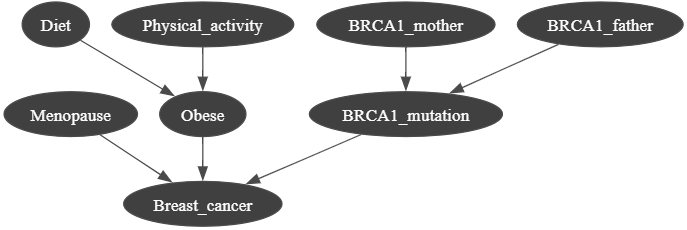
\includegraphics[width=\textwidth]{../figures/Assignment1_network_topology.png}
    \caption{The topology of the bayesian network from assignment 1}
    \label{fig:topology_assingment1}
\end{figure}
This network will be used to generate samples from various sizes, ranging from 100 to 10000 samples. The samples will be generated using the \textit{BNDatabaseGenerator} class from the pyAgrum library.
Next we will perform experiments to see how well the structure of the original network can be learned from the generated samples. For each experiment we will vary 2 parameters: the sample size and the learning algorithm.
The learning algorithms we will use are the Mutual Information-based Incremental Construction (MIIC) algorithm as a constraint-based method, and the greedy hill climbing algorithm (GHC) as a score-based method.
For each experiment, the resulting networks will be compared to the original network to determine how well the topology of the original network is learned. 
This will be a visual comparison and for this the \textit{getBNDiff} method from the \textit{$bn\_vs\_bn$} pyAgrum module will be used.
\textit{getBNDiff} visualizes the differences between two Bayesian networks by highlighting the differences in the structure of the networks.
\begin{figure}[H]
    \centering
    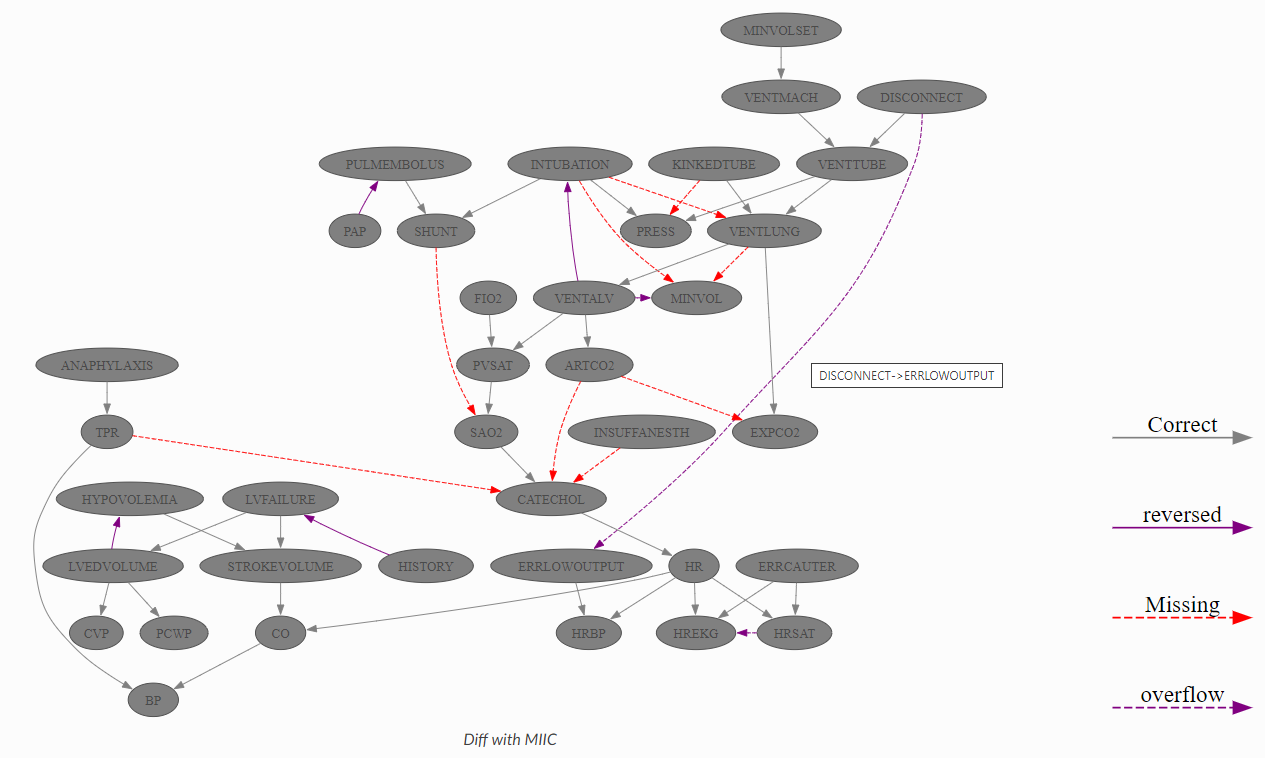
\includegraphics[width=\textwidth]{../figures/getBNDiff_example.png}
    \caption{Example of the getBNDiff visualizations}
    \label{fig:getbndiff}
\end{figure}
\subsection{Learning a classifier}
In the second part we will learn a classifier for breast cancer using Bayesian networks.
\begin{figure}[H]
    \centering
    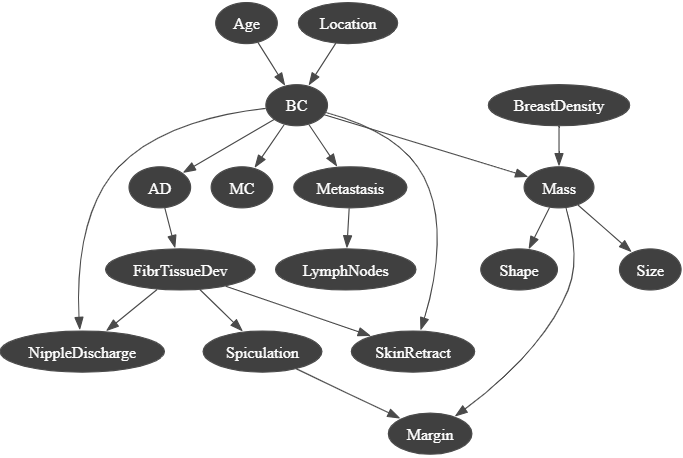
\includegraphics[width=\textwidth]{../figures/Breast_cancer_network_topology.png}
    \caption{The topology of the breast cancer network}
    \label{fig:top_breast}
\end{figure}
We want to compare the difference in performance between a network learned from data and a network constructed based on expert knowledge.
Given is a breast cancer network based on expert knowledge and it will serve as a benchmark to compare our learned network with.
Again using the GHC algorithm, a network structure will be derived from the available breast cancer dataset.
To test the generalization properties of the learned network, we first need to split the dataset into a training and a test set, this to avoid overfitting on the training data.
To quantify the similarity between the learned network and the expert-constructed network, we will use the structural Hamming distance. 
This distance metric measures the number of edges that differ between two networks.
Additionally, the classification performance of both networks will be evaluated in terms of the area under the Receiver Operating Characteristic (ROC) curve,
treating the classification problem as binary (no breast cancer vs. breast cancer).
Finally, we will explore whether incorporating structural constraints can steer the learning algorithm closer to the benchmark network and how this influences classification performance.
This will be done by adding mandatory arcs to the learning algorithm, which will force the algorithm to include these arcs in the learned network.

\section{Results}
\subsection{Investigating the effect of sample size on learning structure}
The visualizations of the differences between the learned networks and the original network can be found in appendix \ref{appendix:raw}.
After 100 samples both the MIIC and the GHC algorithms have a hard time learning the original network structure, 
not even one arc is correct in the network structure generated by the GHC algorithm.
We see a major improvement after 500 samples, where the GHC algorithm already has 5 out of 7 arcs in the correct position, and 4 out of 7 arcs in the correct causal direction.
The MIIC algorithm also has 5 out of 7 arcs in the correct position, but only 3 out of 7 arcs in the correct causal direction. 
Although there are less arcs in the correct causal direction, do notice that the MIIC algorithm does not have any faulty arcs compared to the GHC algorithm.
Next using 1000 samples the GHC algorithm has found all of the correct arcs, but has also introduced 2 faulty arcs. Additionally, there are only 2 arcs in the correct causal direction, which is worse compared to the 500 sample experiment. 
Using 1000 samples the MIIC now has the upperhand as all of the arcs are in the correct position, there are no faulty arcs and 5 out of 7 arcs are in the correct causal direction.
It takes 10000 samples for the GHC algorithm to have all 7 arcs in the correct position, but even then there is still a faulty arc and almost half of the arcs is still pointing in the wrong direction.
There is little improvement when using more than 1000 samples for the MIIC algorithm, when we reach 5000 samples, only one extra arc is in the correct causal direction, and 10000 samples does not improve this further.
\subsection{Learning a classifier}
% What are your findings?

\section{Conclusions and discussion}
% Your conclusions and some reflection on the results. Eg. If you observe unexpected results, can you think of an explanation?
\subsection{Investigating the effect of sample size on learning structure}
The GHC algorithm performed better than the MIIC algorithm when using small sample sizes $<1000$. This could be due to the conservative nature of the MIIC algorithm, to only link nodes based on statistical tests.
This is also reflected in the fact that the MIIC algorithm did not introduce any faulty arcs, while the GHC algorithm did. The GHC algorithm is not dependant on these statistical tests, and only tries to maximize a scoring function.
This is more of a greedy approach and could explain why the GHC algorithm performed better with small sample sizes. Using sample sizes of $1000$ and up, the MIIC algorithm had the best performance by far.
\subsection{Learning a classifier}




% What are the implications of the findings?


% \begin{table}[H]
%     \centering
%     \caption{Variable Description}
%     \label{tab:variables}
%     \begin{tabular}{|c|c|c|}
%         \hline
%         \textbf{Name} & \textbf{Type} & \textbf{Domain} \\
%         \hline
%         Breast cancer & Categoric & \{Yes, No\} \\
%         Menopause & Categoric & \{Before, After\} \\
%         Obese & Categoric & \{No, Moderate, Severe\} \\
%         Diet & Categoric & \{Unhealthy, Normal, Healthy\} \\
%         Physical activity & Categoric & \{None, Little, Regular\} \\
%         BRCA1-mutation & Categoric & \{Yes, No\} \\
%         BRCA1-father & Categoric & \{Yes, No\} \\
%         BRCA1-mother & Categoric & \{Yes, No\} \\
%         \hline
%     \end{tabular}
% \end{table}

\appendix
\section{Appendix} \label{appendix:raw}
\begin{figure}[H]
    \centering
    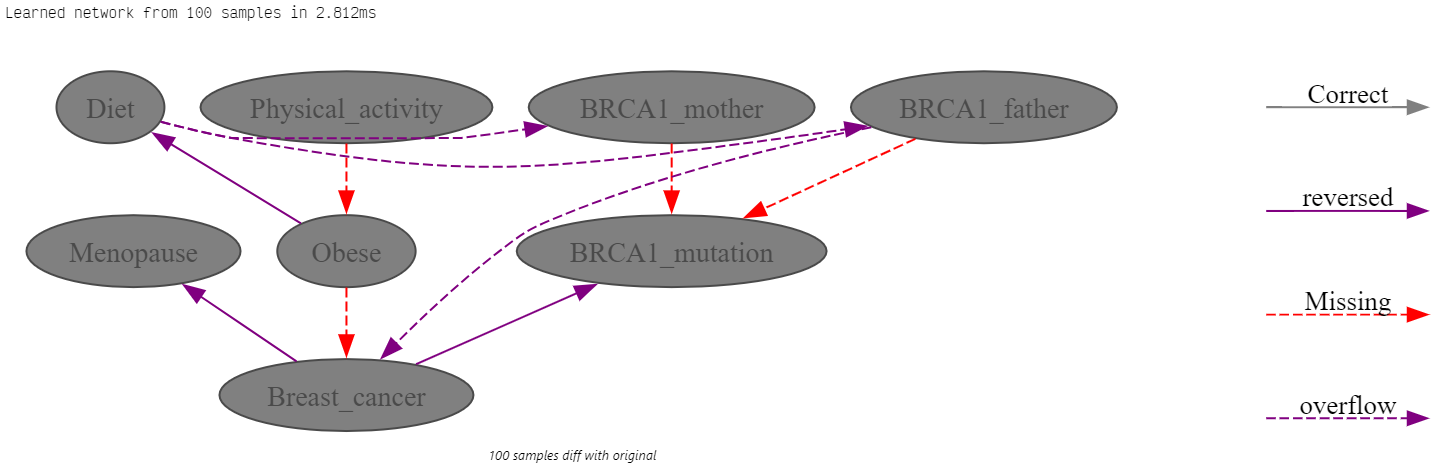
\includegraphics[width=\textwidth]{../figures/greedy_hill_100.png}
    \caption{Greedy Hill Climbing algorithm using 100 samples}
    \label{fig:ghc100}
\end{figure}
\begin{figure}[H]
    \centering
    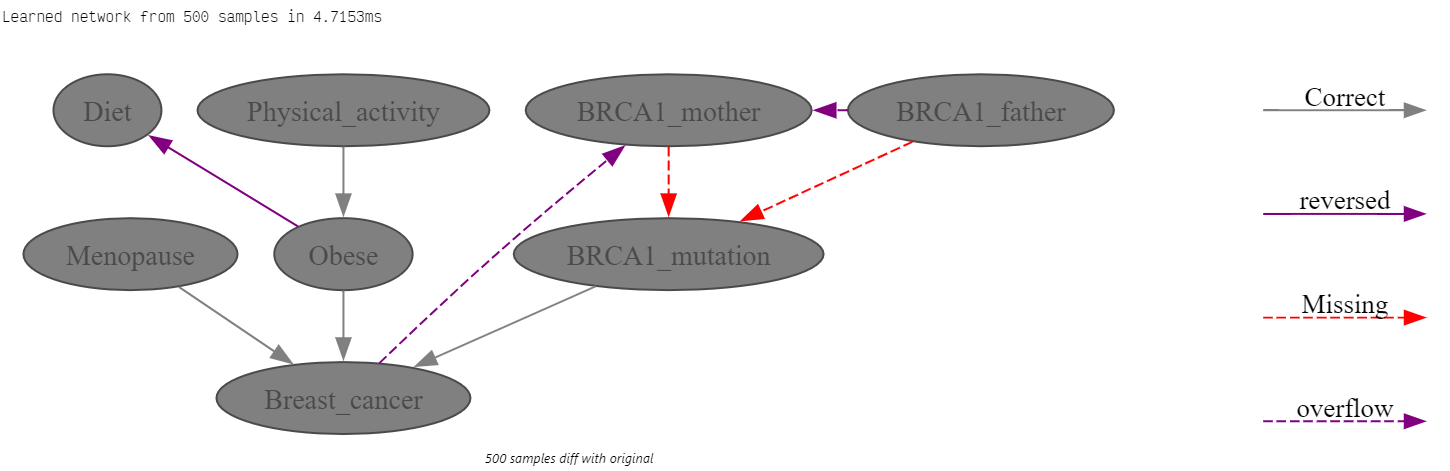
\includegraphics[width=\textwidth]{../figures/greedy_hill_500.png}
    \caption{Greedy Hill Climbing algorithm using 500 samples}
    \label{fig:ghc500}
\end{figure}
\begin{figure}[H]
    \centering
    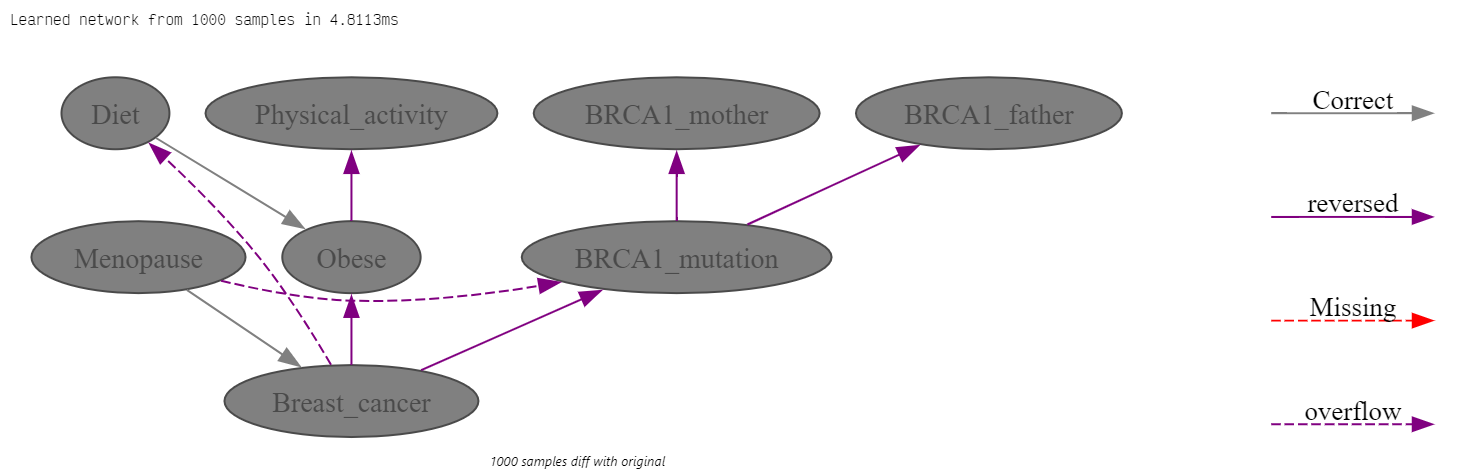
\includegraphics[width=\textwidth]{../figures/greedy_hill_1000.png}
    \caption{Greedy Hill Climbing algorithm using 1000 samples}
    \label{fig:ghc1000}
\end{figure}
\begin{figure}[H]
    \centering
    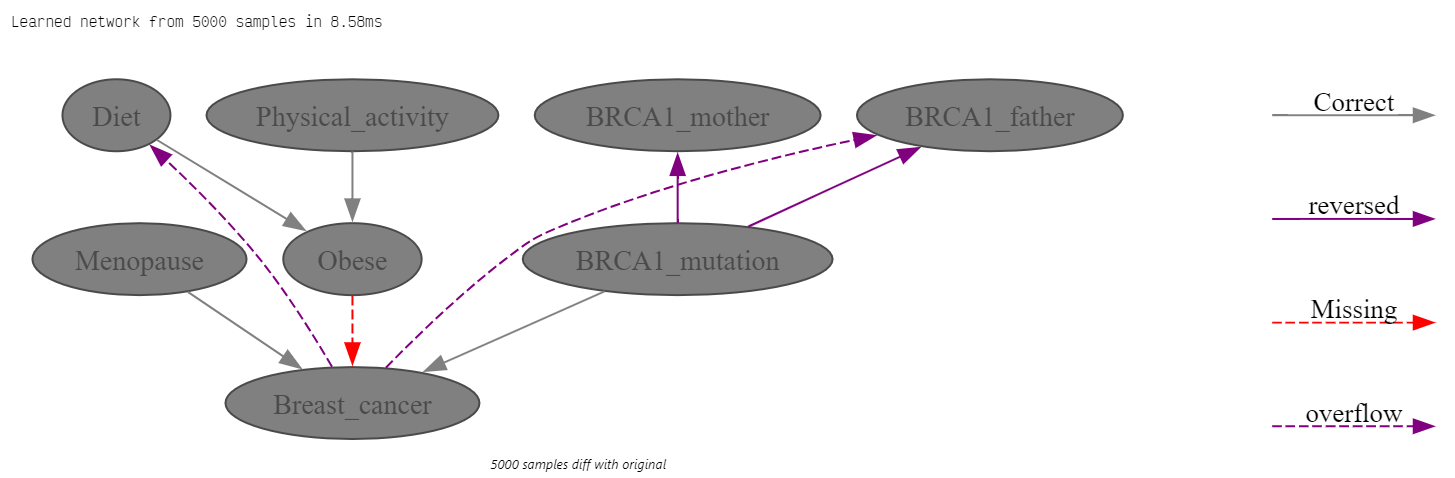
\includegraphics[width=\textwidth]{../figures/greedy_hill_5000.png}
    \caption{Greedy Hill Climbing algorithm using 5000 samples}
    \label{fig:ghc5000}
\end{figure}
\begin{figure}[H]
    \centering
    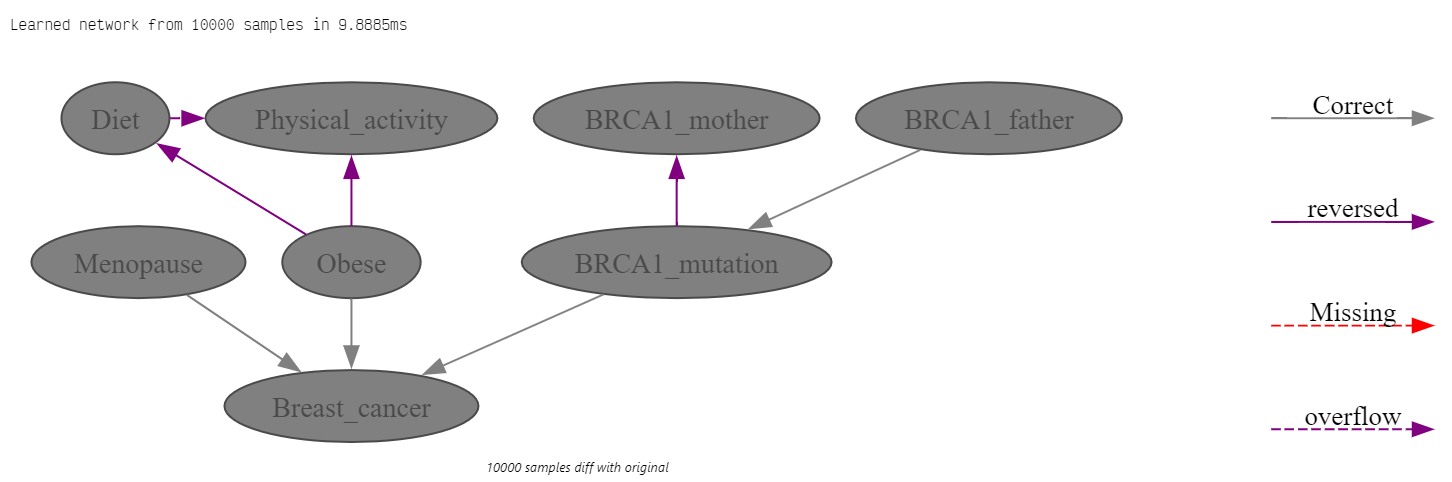
\includegraphics[width=\textwidth]{../figures/greedy_hill_10000.png}
    \caption{Greedy Hill Climbing algorithm using 10000 samples}
    \label{fig:ghc10000}
\end{figure}
\begin{figure}[H]
    \centering
    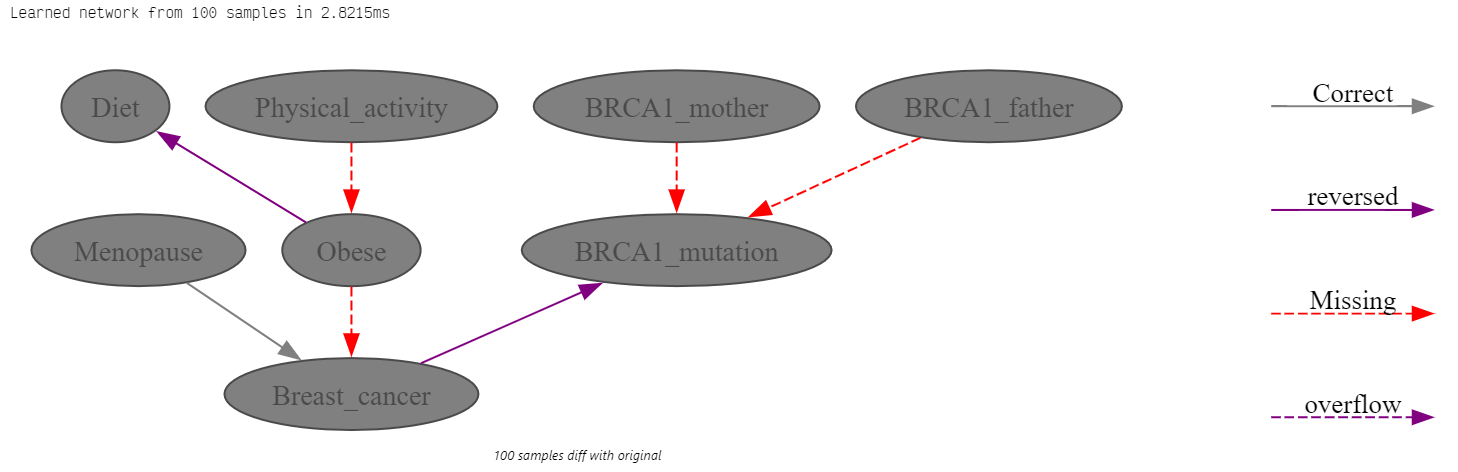
\includegraphics[width=\textwidth]{../figures/MIIC_100.png}
    \caption{MIIC algorithm using 100 samples}
    \label{fig:MIIC100}
\end{figure}
\begin{figure}[H]
    \centering
    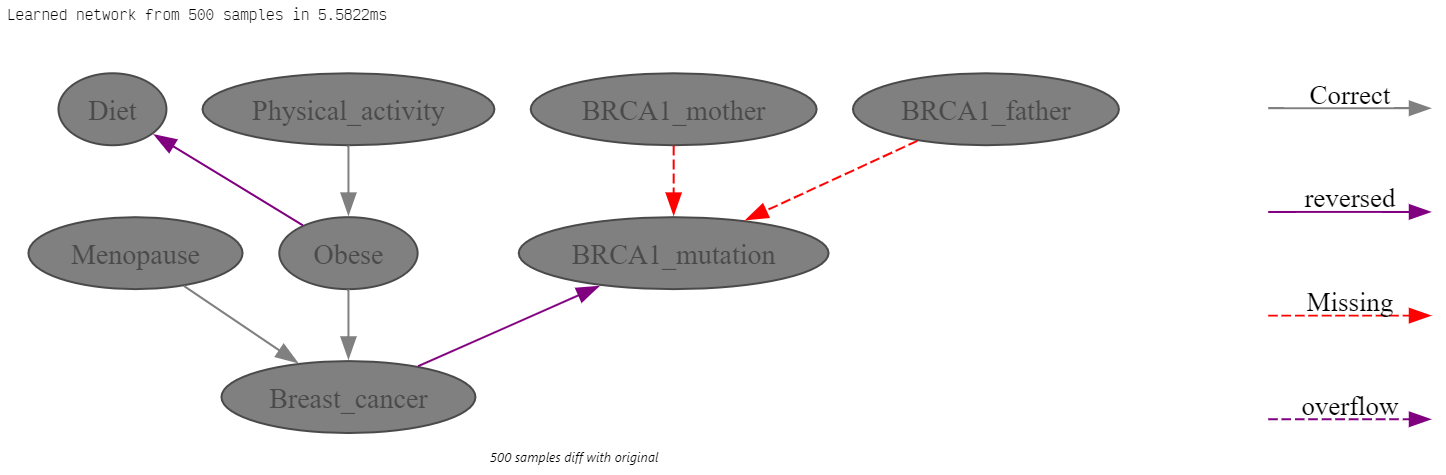
\includegraphics[width=\textwidth]{../figures/MIIC_500.png}
    \caption{MIIC algorithm using 500 samples}
    \label{fig:MIIC500}
\end{figure}
\begin{figure}[H]
    \centering
    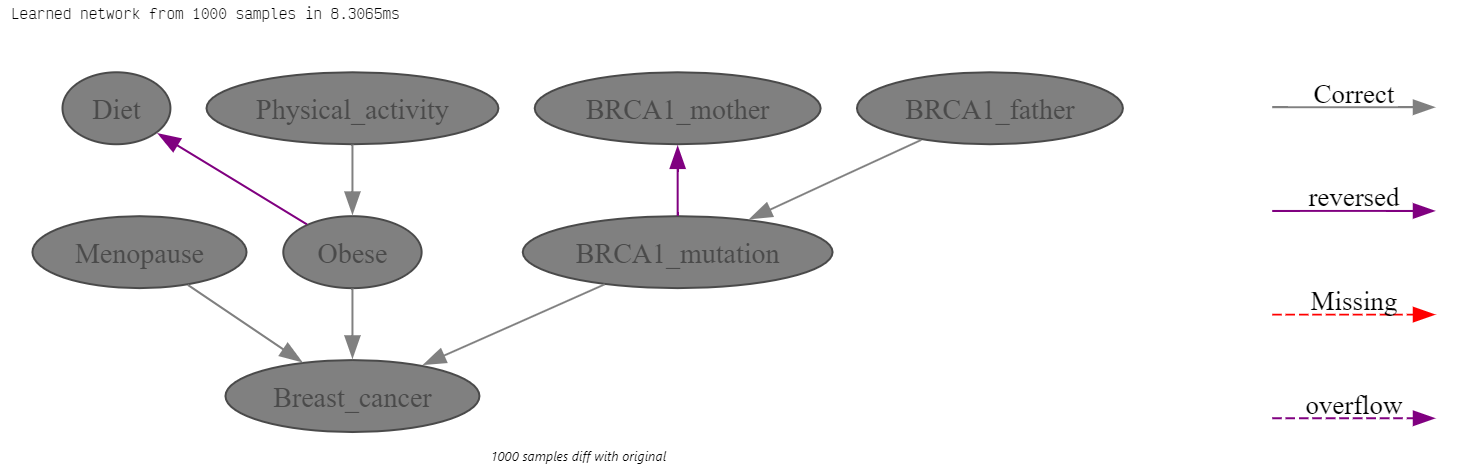
\includegraphics[width=\textwidth]{../figures/MIIC_1000.png}
    \caption{MIIC algorithm using 1000 samples}
    \label{fig:MIIC1000}
\end{figure}
\begin{figure}[H]
    \centering
    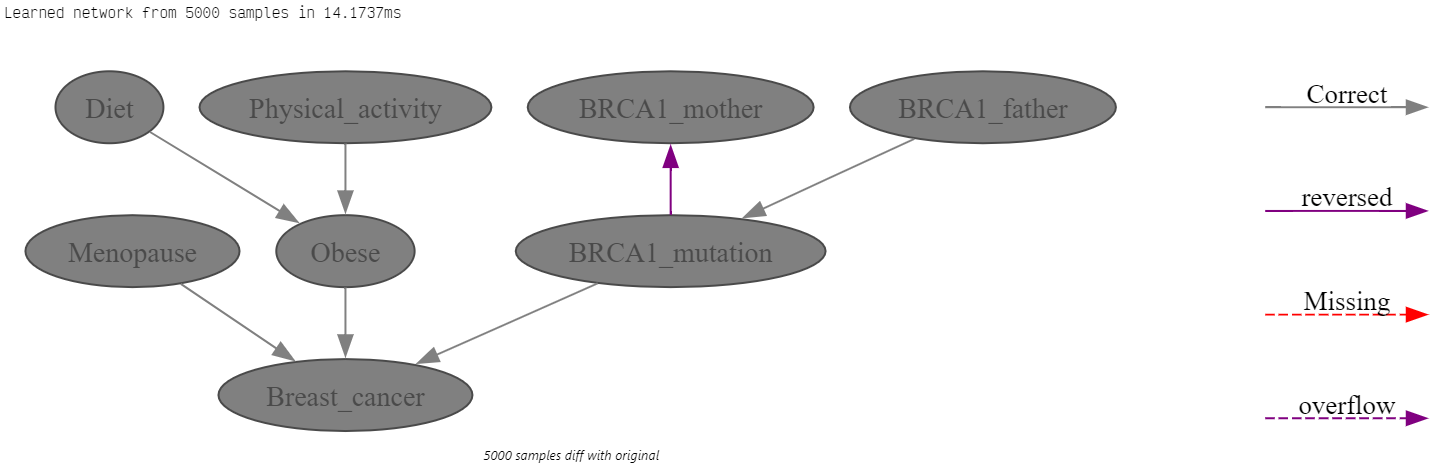
\includegraphics[width=\textwidth]{../figures/MIIC_5000.png}
    \caption{MIIC algorithm using 5000 samples}
    \label{fig:MIIC5000}
\end{figure}
\begin{figure}[H]
    \centering
    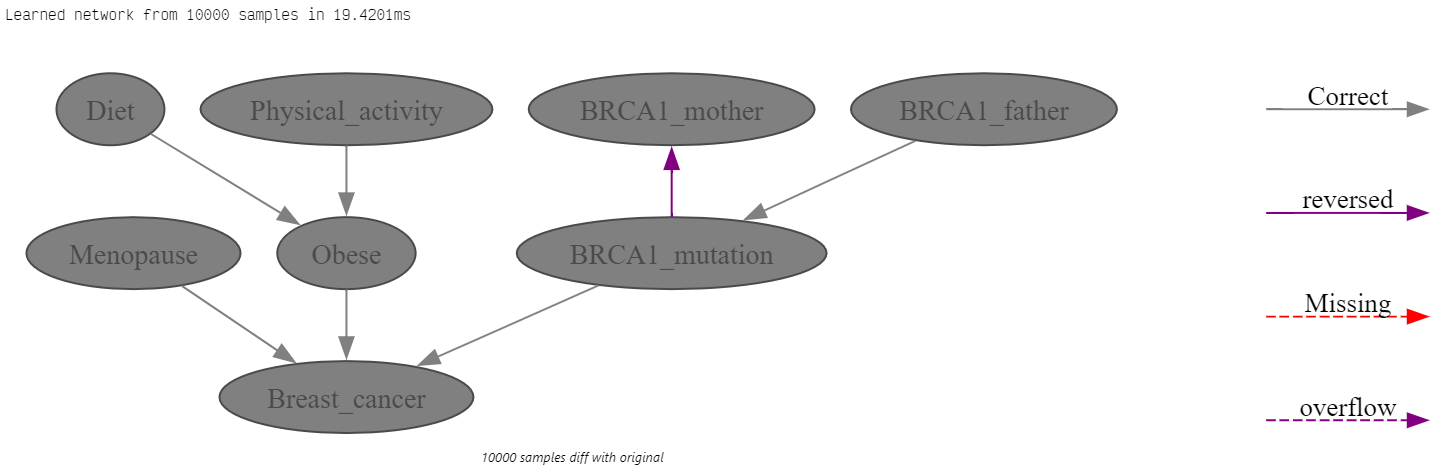
\includegraphics[width=\textwidth]{../figures/MIIC_10000.png}
    \caption{MIIC algorithm using 10000 samples}
    \label{fig:MIIC10000}
\end{figure}
\section{References}
\bibliographystyle{plain}
\bibliography{references}

\end{document}